\subsection{Arduino Nano 33 BLE}

\begin{figure}[h!]
	\centering
 	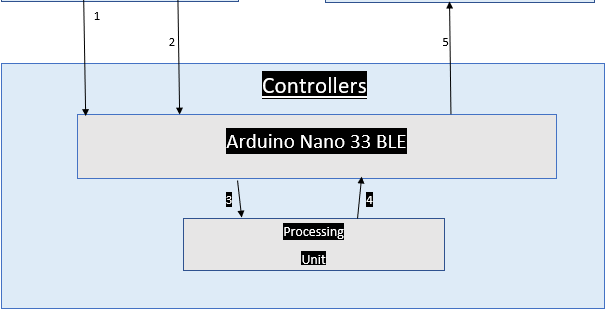
\includegraphics[width=0.60\textwidth]{images/Controller subsystems}
 %\caption{Example subsystem description diagram}
\end{figure}

\subsubsection{Assumptions}
Not applicable

\subsubsection{Responsibilities}
The main responsibility of Arduino nano is to receive anlog signals from temperature sensor and IMU sensore. CPU inside then process analog data then transfers process data to UI/UX layer via bluetooth. 

\subsubsection{Subsystem Interfaces}
data elements will pass through this interface.

\begin {table}[H]
\caption {Subsystem interfaces} 
\begin{center}
    \begin{tabular}{ | p{1cm} | p{6cm} | p{3cm} | p{3cm} |}
    \hline
    ID & Description & Inputs & Outputs \\ \hline
    & Controller interface & \pbox{3cm}{input 1 \\ input 2 \\ input 4} & \pbox{3cm}{output 5}  \\ \hline
    \end{tabular}
\end{center}
\end{table}

\subsection{Processing Unit}

\begin{figure}[h!]
	\centering
 	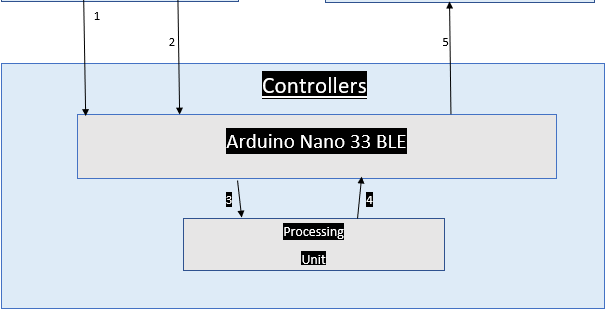
\includegraphics[width=0.60\textwidth]{images/Controller subsystems}
 %\caption{Example subsystem description diagram}
\end{figure}

\subsubsection{Assumptions}
Hydrometer is always turned on whenever it's inside the fermentation vessel. Since, position of hydrometer is needed for specific gravity, it's assumed that the hydrometer is floating.

\subsubsection{Responsibilities}
60 MHz CPU is responsible for processing temperature and specific gravity data, that it receives from sensors attached to Arduino nano. Arduino nano is programmed to handle those data whenever nano is turned on. It outputs the accurate temperature and specific gravity data after processing.

\subsubsection{Processing Unit Interface}

\begin {table}[H]
\caption {Subsystem interfaces} 
\begin{center}
    \begin{tabular}{ | p{1cm} | p{6cm} | p{3cm} | p{3cm} |}
    \hline
    ID & Description & Inputs & Outputs \\ \hline
    & Processing Unit Interface & \pbox{3cm}{input 3} & \pbox{3cm}{output 4}  \\ \hline
    \end{tabular}
\end{center}
\end{table}